\section{Patterns 8 - Redegør for følgende concurrency mønstre}

\subsection{Fokuspunkter}

\begin{itemize}
	\item Parallel Aggregation.
	\item MapReduce.
\end{itemize}

\subsection{Parallel Aggregation}
I forlængelse af parallelle loop kan det sige at ikke alle PL's iterationer eksekveres uafhængigt. Fx et loop der udregner en sum, bruger hver iterations resultat til at akkumulere en enkelt variabel der indeholder den udregnede sum op til det iterationsniveua vi er på. Denne akkumulerede værdi er en aggregation.

Man Skulle dermed tro at at aggregation operation ikke kan forenees med \textit{parallel loops}. Dog findes der en vej! Parallell aggregation pattern!

Dette pattern benytter \textit{unshared} lokale variabler som merges til slut for at give det endelige resultat. PA kaldes også parallel reduction pattern, idet den kombinerer flere inputs til et enkelt output.\\

\subsubsection{Eksempel med summering}
Tag eksempelvis summeringen af nogle tal vist i ligning~\ref{eq:pl1}:
\begin{equation}\label{eq:pl1}
sum = a + b + c + d
\end{equation}

Istedet for at løse dette sekventielt, som det i ligning~\ref{eq:pl2} bliver demonstreret. 
\begin{equation}\label{eq:pl2}
=((a + b) + c) + d
\end{equation}

Så kan vi ved at bruge Parallel Aggragation gøre som ligning~\ref{eq:pl3} giver udtryk for.
\begin{equation}\label{eq:pl3}
=(a + b) + (c + d)
\end{equation}

Den sidste metode vist i ligning~\ref{eq:pl3} kan vi bruge parallelt og dette er meningen med Parallel Aggregation!\\

En illustrering af dette har vi i figur~\ref{fig:reduce}, hvordan man igen kan se hvordan paralleliseringen af løsningen kan være simpel og effektiv på samme tid.

\newcommand{\si}{5cm}
\begin{figure}[H]
	\centering
	\begin{minipage}{.49\textwidth}
		\centering
		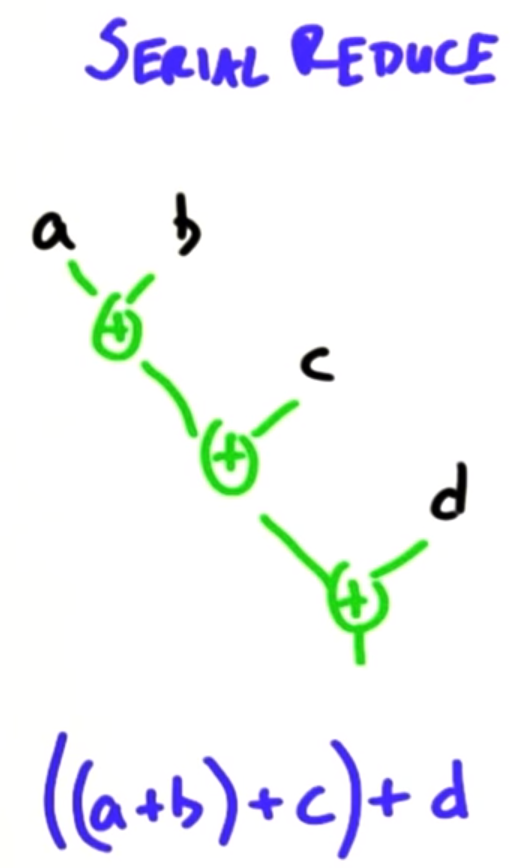
\includegraphics[height=\si]{figs/aggregation/seqReduce}
		%\captionof{figure}{Sekventiel reducering}
		\label{seqReduce}
	\end{minipage}
	\begin{minipage}{.49\textwidth}
		\centering
		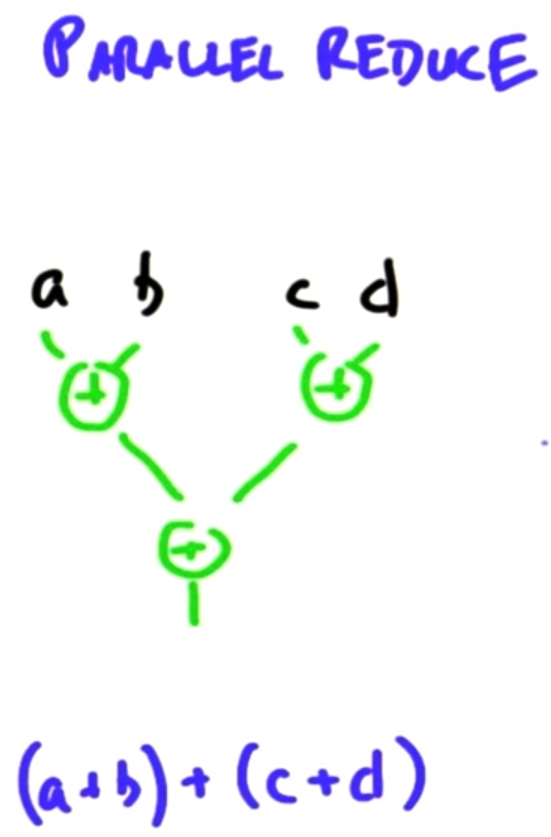
\includegraphics[height=\si]{figs/aggregation/paraReduce}
		%\captionof{figure}{Parallel reducering}
		\label{paraReduce}
	\end{minipage}
	\caption{Forskellen på seriel og parallel reducering.}
	\label{fig:reduce}
\end{figure}

\subsection{MapReduce}
MapReduce er en måde at arbejde på meget store datasæt. Der arbejdes med MapReduce parallelt på dataen.

\subsubsection{4 steps}
Vi kan opdele MapReduce modellen i 4 steps som for vores eksempel bruges til at finde ud af hvor mange af hver kulør der findes i vores stak med spillekort.

\begin{enumerate}
	\item \textbf{Distribuer source data til forskellige nodes.}\\
	Fordel stakken af kort ud på alle noder.
	\item \textbf{Map data - Repræsenter data i key-value par.}\\
	Hver node tæller hvor mange af hver kulør den har fået tildelt. Dette repræsenteres med key-value par. eg. Kulør (key) og kortværdi (value).
	\item \textbf{Gruppér data.} \\
	Grouperen har til ansvar at gruppere mappernes key-value par. Her tages alle klør par og sættes i samme gruppe, alle ruder par sættes sammen osv.
	\item \textbf{Reducer eller merge  data fra grouperen.}\\
	Her tælles sammen hvor mange af hver kulør der er i de grupperede data.
\end{enumerate}
